\infolevone{

\subsection{High Voltage Supplies and Control}
\label{sec:highvoltage}

\paragraph{Overview}
}
\infoleveqnull{
\section{Detector High Voltage}
}
All of the detector systems in Hall C use high voltages, from hundreds to
several thousand volts, to either power photomultiplier tubes or maintain
electric fields around sense wires in drift chambers.
These include scintillators, drift chambers,
scintillators, shower detectors, and aerogel Cherenkovs.

\begin{safetyen}{0}{0}
\infoleveqnull{\subsection{Hazards}}
\infolevone{\subsubsection{Hazards}}

The personnel hazard with these devices is the high voltage.
This qualifies as a Class I electrical hazard due to the supplies providing
voltage $>$50\,VDC with current limited to $\leq 5$\,mA.\footnote{JLab ES\&H
  Manual, Chapter 6230 - Appendix T1 - ``Determining Equipment Class and Work
  Modes"}
This same hazard can
damage phototubes if voltage is left on when tubes are exposed to room
lighting.

\infoleveqnull{\subsection{Mitigations}}
\infolevone{\subsubsection{Mitigations}}
\begin{itemize}
  \item All user configurable high voltage cabling/patching is made with
  coaxial cables rated for high voltage with SHV connectors.
  \item High voltage shall be turned off before disconnecting (or connecting)
  high voltage cables from (or to) phototubes, power supplies or patch panels.
  \item High voltage shall be turned off and high voltage cables shall
  be removed from phototubes before handling phototubes or the detector
  elements they are used with.
  \item Current limits are set on power supplys to trip high voltage in case
  of shorts or shocks.
  \item External metal parts of detectors such as mu-metal shields are wrapped
  with electrical tape.  Exposed metal parts are grounded through both the HV
  cable and signal cable grounds.
\end{itemize}

\infoleveqnull{\subsection{Responsible Personnel}}
\infolevone{\subsubsection{Responsible Personnel}}

The individuals responsible for the operation
of the high voltage system are shown in Table \ref{tab:scin:personnel}.

\begin{namestab}{tab:scin:personnel}{Detector high voltage responsible personnel} {%
      Detector high voltage responsible personnel.}
  \StephenWood{}
  \MahlonLong{}
  \JoeBeaufait{}
  \JackSegal{}
\end{namestab}
\end{safetyen}

\infolevone{
% The next two should be combined with the
All the detector elements in the SHMS and HMS require the use of High Voltage. The
high voltage supplies for the detectors are located in the
electronics room and second floor of the counting house. They are connected to
the detector shield houses through multiconductor high voltage patch systems,
and to the detectors through coaxial cables with SHV connectors.
During experiments the control of the high voltage supplies is
done remotely via any of the computers at the console
the Hall~C counting house.

As a general rule no work should be done on detectors which are under
High Voltage and
High Voltage cables should never be removed or installed while the supply is on.

\subsubsection{High Voltage Configuration and Operation}
The CAEN Distributed High Voltage System is responsible for
providing high voltage power to all HMS and SHMS detector systems.
This system is a
networked system made up of individual crates (Controllers)
each of which can hold several independent high voltage modules
(Cards).  The crates are a mix of SY403 mainframes which hold four cards
with 16 SHV outputs and newer SY4527 mainframes holding up to 8 cards with 24
SHV outputs each.  (Other cards with different numbers of channels and
different high voltage connector form factors are available, but only
the described types are currently used in Hall C.)
There are several flavors of cards in use with the
Hall~C detector systems which are listed in Tables~\ref{tab:hv_cards}
and \ref{tab:hv_cards_new}.  A given crate may have a mix of card
types, although cards can not be exchanged between SY403 and SY4527 crates.

\begin{table}
\caption{Specifications of SY403 High-Voltage Cards used in Hall~C Detector
Systems\label{tab:hv_cards}.}
\begin{center}
\begin{tabular}{ccccc}
        &Card type      &Max Voltage    &Max Current    &Detector System \\
	&		&		&		&	\\
	& A403 (or A503)&--3000V	&3.0mA		&Hodo/Shower\\
	& A503P		&+3000V		&3.0mA		&Cherenkov/Aerogel\\
	& A505		&--3000V	&200$\mu$A 	&Drift Chambers\\
  \end{tabular}
\end{center}
\end{table}

\begin{table}
\caption{Specifications of SY4527 High-Voltage Cards used in Hall~C Detector
Systems\label{tab:hv_cards_new}.}
\begin{center}
\begin{tabular}{ccccc}
  &Card type      &Max Voltage    &Max Current    &Detector System \\
  &		&		&		&	\\
  & A1535SN       &--3500V	&3.0mA		&Hodo/Shower/Heavy Gas\\
  & A1535SP       &+3500V    &3.0mA		&Noble Gas/Aerogel\\

  \end{tabular}
\end{center}
\end{table}

The system is typically controlled through EPICS.  Various methods of
direct/local control are available for the two different crate types.

%\begin{figure}
%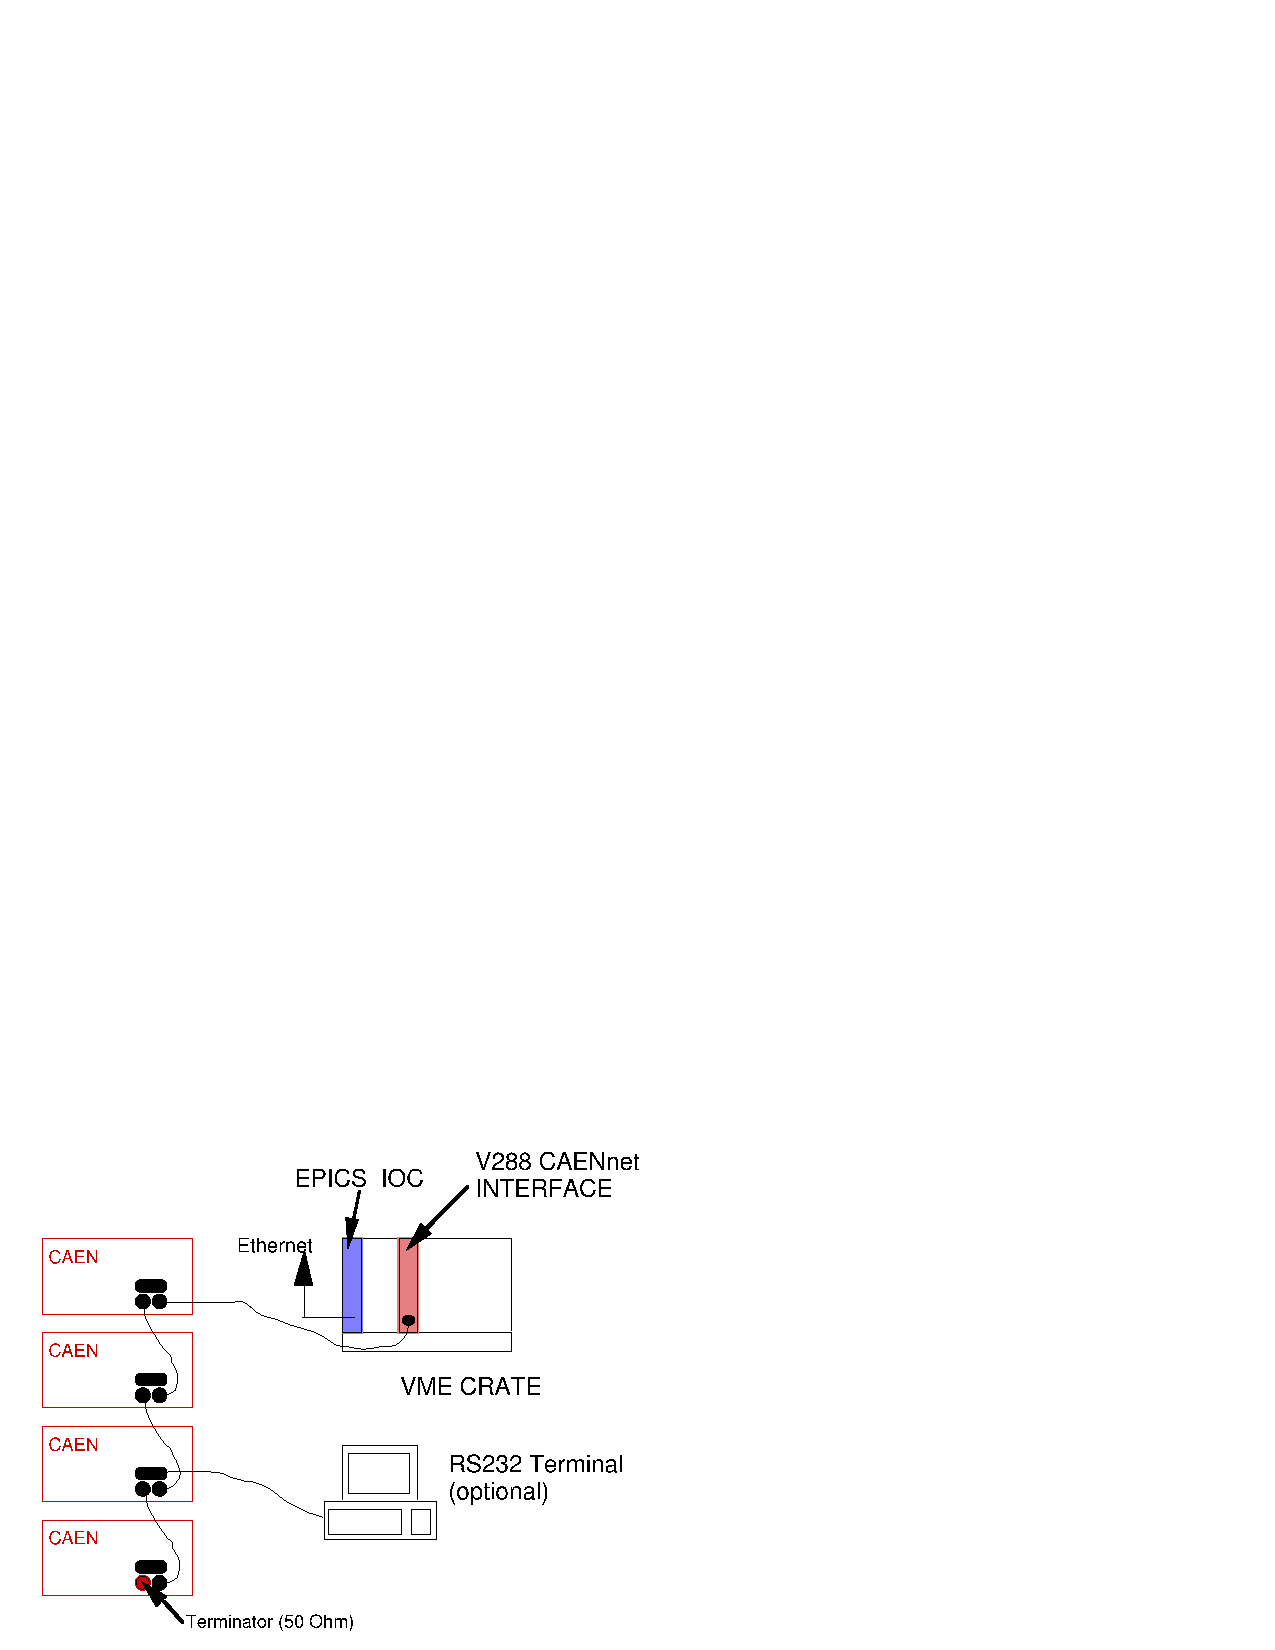
\includegraphics[height=4.5in]{CAENHV.pdf}
%\caption{Generic CAEN High Voltage System setup\label{fig:caen_setup}}
%\end{figure}

HV channel assignments currently in effect are indicated in
two files (``group\_map'' and
``channel\_map'') in the directories \$EPICSHL/HV/hms\_all (for HMS) and
\$EPICSHL/HV/shms\_all (for
SHMS) when logged in as cvxwrks to one of the cdaq machines.

%\vfil\eject
\paragraph{General Operation}

\subparagraph{Normal Operation:}

In general the high voltage system will be controlled or monitored
from the counting house using the EPICS slow control system.
Operation of the EPICS graphical interfaces is described in the CAEN
HV Operation Howto~\cite{howto:CAEN_HV_operation}.

In case of a dead high voltage channel, the high voltage cable for a
given detector element can be moved
to a spare high voltage channel, if available.  (The channel\_map
file, described above shows which channels are in use.)  Care must be
taken to always use the correct type of HV (positive vs. negative,
vs. drift chamber supply).  The procedure to make these changes is
described in the CAEN HV Operation
Howto~\cite{howto:CAEN_HV_operation}.  Any changes in HV configuration
shall be documented in the logbook.

For more complicated changes to the HV configuration, such as changing or
adding HV cards or mainframes, consult and expert and the Caen High
Voltage System EPICS Controls Expert Howto~\cite{howto:CAEN_HV_expert}.

\subparagraph{Important Features:}

The user can program several important features for individual
cards and/or channels.  The most common are:

\begin{itemize}
\item{HV limits -- 2 types including a hardware maximum (common to a
card) set with a pot on the front panel of each card and a software
maximum for each channel.}
\item{Current Trip Value -- The current over which the system will
indicate an alarm status and initiate a trip off of that channel.}
\item{Current Trip Time -- The amount of time the system will allow
the alarm condition before actually switching off that channel.}
\item{Ramp-up Value -- The number of volts/sec the voltage will ramp
to its set point upon switching on the channel.}
\item{Other Features -- See the CAEN Technical Information Manual.}
\end{itemize}

\subparagraph{Direct/Local Operation}
The SY403 mainframes may be controlled through the front panel or an
RS232 interface, while the SY4527 The high voltage main frames can be
controlled through a web interface.   These methods of control are
described in the CAEN HV Operation
Howto~\cite{howto:CAEN_HV_operation} and the vendor manuals for the
SY403~\cite{caensy403manual} and SY4527~\cite{caensy4527manual}.
These modes of control are meant for
diagnostics and testing of a detector system prior to running.

\paragraph{Safety Concerns/Caveats}

There are a number of cautions one should observe when operating
the CAEN HV equipment to avoid damage and insure proper functioning:

\begin{itemize}
\item{Use only proper SHV connectors and approved cables when
connecting equipment to the supply.}
\item{{\bf DO NOT} attach/remove HV cables when loads are present on the
channel ( a red LED above each channel indicates the presence of a
load).}
\item{Insure adequate ventilation around crates to avoid overheating
of the electronics.}
\item{Wait 2-3 minutes after switching off a crate before removal of a
HV card.}
\item{Insure proper static precautions when handling HV cards.}
\end{itemize}

For proper EPICS control operation (SY403):

\begin{itemize}
\item{Inter-crate connections must be unbroken and terminated at the
last crate at 50 Ohms.  All crates must be powered on.}
\item{Crate numbers for each crate in the chain must be distinct and
different from 0 (i.e. 1-99)}
\item{The HV Enable switch (on the front panel of each crate) must be on.}
\item{One should refrain from any local operation of crates when the
EPICS system is active.}
\end{itemize}
}

\subsubsection{High Voltage System Checkout}
\label{sec:highvoltagecheckout}

Before starting an experiment, or before using the high voltage system to
test detectors, proper functioning of the HV supplies and EPICS controls
should be verified with this checklist.
\begin{itemize}
  \item{Check EPICS: Using the EPICS Control system as described in the CAEN HV
  Operation Howto~\cite{howto:CAEN_HV_operation}, verify that voltage set
  points and current/voltage limits are read by the control system.}
  \item{Verify Operation: For the detector(s) of interest, individually
  turn on each channel.  Verify that the channel reaches the desired
  set voltage.  If the readback voltage exceeds the set voltage by more
  than a few volts
  (Overvoltage), or fails to reach full voltage (Undervoltage), immediately
  turn off the channel, report the observation in the logbook and consult
  an expert.}
  \item{Verify Limits: Make a backup of HV settings.  For each channel in the
  detector, set a current limit below the current being drawn by the detector
  channel.  Verify that each channel trips.  Similarly, set a maximum voltage
  for each channel below the set point and verify that the voltage limit
  is enforced.  (This may change voltage set points, so they may need to
  be restored from backup.)  Consult an expert if any channels fail to trip
  on overcurrent or if maximum voltage is not enfored.}
  \item{Interlocks: If any high voltage systems are interlocked with other
  systems, verify that assertion of the interlock signal turns off high
  voltage.}
\end{itemize}
